\documentclass[conference]{IEEEtran}
\IEEEoverridecommandlockouts
% Based on the IEEE Conference Template (Overleaf). Compile with pdfLaTeX (Overleaf default) or tectonic.
\usepackage[T1]{fontenc}
\usepackage{cite}
\usepackage{amsmath,amssymb,amsfonts}
\usepackage{algorithm}
\usepackage{algpseudocode}
\usepackage{graphicx}
\usepackage{textcomp}
\usepackage{xcolor}
\usepackage{booktabs}
\usepackage{url}
\usepackage{tikz}
\usetikzlibrary{arrows.meta,positioning,fit,calc}
\usepackage[hidelinks]{hyperref}
\graphicspath{{figures/}}
\newcommand{\figref}[1]{Fig.~\ref{#1}}
\DeclareMathOperator{\clip}{clip}
% Many full-width figures: allow more pending floats and fuller float pages.
\extrafloats{100}
\renewcommand{\topfraction}{0.9}\renewcommand{\dbltopfraction}{0.9}
\renewcommand{\textfraction}{0.07}\renewcommand{\floatpagefraction}{0.75}\renewcommand{\dblfloatpagefraction}{0.75}

\begin{document}

\title{MARS-O-RAN: Mission-Aware, Risk-Aware Elastic Network Slicing for Emergency Robotics in an O-RAN Digital Twin}

\author{\IEEEauthorblockN{Ishaan Jayaram Shetty}
\IEEEauthorblockA{\textit{Dept. of Electronics and Communication Engg.} \\
\textit{IIIT Dharwad}\\
Dharwad, India}
\and
\IEEEauthorblockN{Prashant Kumar}
\IEEEauthorblockA{\textit{Dept. of Electronics and Communication Engg.} \\
\textit{IIIT Dharwad}\\
Dharwad, India}
\and
\IEEEauthorblockN{Himanshu Kumar Sonkar}
\IEEEauthorblockA{\textit{Dept. of Electronics and Communication Engg.} \\
\textit{IIIT Dharwad}\\
Dharwad, India}
\and
\IEEEauthorblockN{Naman Kumar}
\IEEEauthorblockA{\textit{Dept. of Computer Science and Engg.} \\
\textit{IIIT Dharwad}\\
Dharwad, India}
}

\maketitle

\begin{abstract}
During an industrial emergency, robots, sensors, and responders share one radio cell, and the traffic that matters most changes as the mission advances. We study a gas-leak response in which five dependent tasks (gas detection, source localization, robot navigation, valve inspection, and valve manipulation) each carry a deadline, a data-freshness limit, and a reliability target. We formulate slice resource allocation as a stochastic, integer, sequential decision problem and propose MARS, a heuristic controller that splits physical resource blocks (PRBs) among four slices using a mission-criticality score, a severity-dependent risk reserve, and stability constraints. MARS is evaluated in a Python digital twin styled after the Open Radio Access Network (O-RAN) control loop against STATIC, PROPORTIONAL, and MISSION-AWARE baselines. Over 30 paired random seeds, both mission-oriented policies raise the task-level success score from 0.187 (STATIC) to above 0.70 and lower mission loss in every seed (Wilcoxon $p<10^{-5}$). Relative to MISSION-AWARE, MARS cuts reconfiguration cost by 43.7\% in all 30 seeds while its mission outcome is statistically indistinguishable. Eleven edge-case studies show that MARS gains up to 8.7 percentage points under mild incidents but loses up to 9 points under tight deadlines and 16 points under heavier workload, and they expose three model properties: an infeasible final task at nominal severity, a radio--edge budget paradox, and saturated criticality weights. All results come from a reproducible simulation, not from field or testbed measurements.
\end{abstract}

\begin{IEEEkeywords}
O-RAN, network slicing, emergency robotics, mission-aware resource allocation, edge computing, Age of Information, CVaR, digital twin.
\end{IEEEkeywords}

%=====================================================================
\section{Introduction}
A ground robot closing a leaking valve, a drone streaming camera frames to an edge server, responders viewing hazard overlays, and a field of gas sensors can all share one private cell during an industrial emergency. Their demands conflict, and which one deserves the spectrum depends on where the mission stands. Camera and sensor uplink dominate while the leak is being located; a few kilobits of control traffic, delivered quickly and reliably, matter more once the robot grips the valve. A slicing policy that looks only at instantaneous traffic volume cannot see this shift.

Open RAN makes application-driven control architecturally plausible. Its RAN Intelligent Controllers (RICs) run control loops at two time scales: a near-real-time RIC that acts on the base station over the E2 interface, and a non-real-time RIC that issues policies over A1 \cite{oranarch,oranwg3,polese}. A mission-aware slicing rule would naturally sit in the near-real-time loop. We study the decision logic of such a rule inside a Python digital twin; no E2 or A1 messages are exchanged and no RIC software is deployed.

We ask two questions. First, \emph{can tying PRB shares to the currently executable mission task improve task completion over fixed or demand-driven slicing?} Second, \emph{under which budgets, incident severities, deadlines, and workloads does that advantage disappear or reverse?} We give the second question as much weight as the first, because a controller tuned at one operating point says little about its behavior elsewhere.

\textbf{Contributions.}
\begin{enumerate}
\item A system model that couples a mission-task dependency graph to four network slices, an analytical radio and edge-compute service model, Age-of-Information (AoI) freshness, and end-to-end reliability (Section~\ref{sec:model}).
\item A formulation of mission-aware slicing as a stochastic integer program with a tail-risk (CVaR) objective term and reconfiguration cost (Section~\ref{sec:problem}).
\item MARS, a low-complexity heuristic controller combining a dynamic criticality score, a severity-dependent risk reserve, a hold time, and a per-step change limit (Section~\ref{sec:mars}).
\item A paired-seed statistical comparison with three baselines using bootstrap confidence intervals and signed-rank tests (Section~\ref{sec:results}).
\item An edge-case study across eleven sweeps that maps where each policy works and traces each failure to a model mechanism (Section~\ref{sec:edge}).
\end{enumerate}

%=====================================================================
\section{Related Work}
\textbf{Open RAN control.} The O-RAN specifications separate a near-real-time controller from a non-real-time one \cite{oranarch,oranwg3}, and Polese \emph{et al.} survey the interfaces and the learning-based applications proposed for both \cite{polese}. Our digital twin mirrors this split only loosely: scenario settings are fixed before a run, playing the role of a slow policy, and a per-second heuristic plays the role of the fast loop.

\textbf{Slicing with guarantees.} Much recent O-RAN slicing work optimizes service-level agreements with reinforcement learning. SafeSlice, for instance, adds a safety layer so that a deep RL agent respects both cumulative and per-step latency limits \cite{safeslice}. Baguer \emph{et al.} show that slicing over Open RAN can sustain beyond-visual-line-of-sight drone operation \cite{bvlos}. Both target per-slice performance; neither models a sequence of dependent tasks whose value changes as the mission advances, which is the gap MARS-O-RAN explores.

\textbf{Freshness, short packets, and tail risk.} We borrow three tools from adjacent fields. Age of Information quantifies how stale the newest delivered update is \cite{kaul,aoi}; a robot steering toward a valve is better served by a recent position than by a large but outdated batch. Finite-blocklength theory shows that short control packets cannot reach Shannon capacity at low error rates \cite{polyanskiy}, which motivates the rate penalty in our radio model. Conditional value at risk (CVaR) summarizes the worst part of a loss distribution and admits a convex reformulation \cite{cvar}; we use it in the problem objective and to score simulated outcomes. Validating our abstractions with a packet-level simulator such as 5G-LENA \cite{lena} remains future work.

%=====================================================================
\section{Problem Scenario and System Model}\label{sec:model}
\subsection{Scenario}
An industrial plant experiences a gas leak at $t_0=20$\,s. A response team deploys a drone camera, a gas-sensor field, an unmanned ground vehicle (UGV) with a manipulator, and responder extended-reality (XR) headsets, all served by one private cell and a co-located multi-access edge computing (MEC) server. The mission is to detect the leak, localize its source, drive the UGV to the valve, inspect it, and close it. \figref{fig:system} summarizes the digital twin.

\begin{figure}[t]
\centering
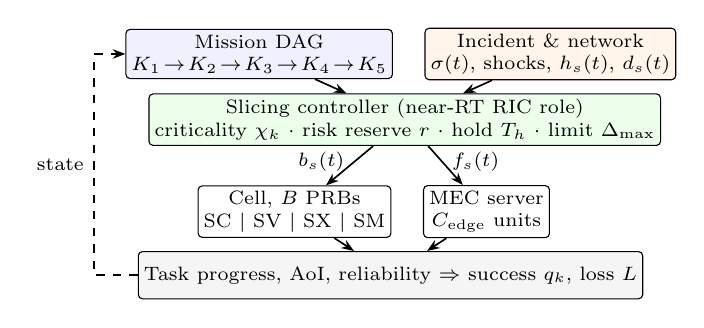
\begin{tikzpicture}[font=\scriptsize, node distance=3mm and 4mm,
  box/.style={draw, rounded corners=1.5pt, align=center, minimum height=6mm, inner sep=2pt},
  arr/.style={-{Stealth[length=1.6mm]}, semithick}]
\node[box, fill=blue!6] (dag) {Mission DAG\\$K_1\!\to\!K_2\!\to\!K_3\!\to\!K_4\!\to\!K_5$};
\node[box, fill=orange!8, right=of dag] (env) {Incident \& network\\$\sigma(t)$, shocks, $h_s(t)$, $d_s(t)$};
\node[box, fill=green!8, below=5mm of $(dag)!0.5!(env)$, minimum width=50mm] (ctl) {Slicing controller (near-RT RIC role)\\criticality $\chi_k$ $\cdot$ risk reserve $r$ $\cdot$ hold $T_h$ $\cdot$ limit $\Delta_{\max}$};
\node[box, below=5mm of ctl, xshift=-14mm] (gnb) {Cell, $B$ PRBs\\SC $\mid$ SV $\mid$ SX $\mid$ SM};
\node[box, right=of gnb] (mec) {MEC server\\$C_{\mathrm{edge}}$ units};
\node[box, fill=gray!8, below=5mm of $(gnb)!0.5!(mec)$, minimum width=50mm] (out) {Task progress, AoI, reliability $\Rightarrow$ success $q_k$, loss $L$};
\draw[arr] (dag) -- (ctl); \draw[arr] (env) -- (ctl);
\draw[arr] (ctl) -- node[left, pos=0.4]{$b_s(t)$} (gnb);
\draw[arr] (ctl) -- node[right, pos=0.4]{$f_s(t)$} (mec);
\draw[arr] (gnb) -- (out); \draw[arr] (mec) -- (out);
\draw[arr, dashed] (out.west) -- ($(dag.west |- out.west)+(-4mm,0)$) |- node[pos=0.25, left]{state} (dag.west);
\end{tikzpicture}
\caption{MARS-O-RAN digital twin. Each 1\,s step the controller observes mission and network state, allocates PRBs $b_s(t)$ (which also set edge shares $f_s(t)$), and the twin updates task progress, freshness, and reliability.}
\label{fig:system}
\end{figure}

\subsection{Network and Slices}
Time is slotted into steps of $\Delta t=1$\,s over a horizon $T=300$\,s. The cell has $B$ PRBs ($B=100$ nominally). Let $b_s(t)\in\mathbb{Z}_{\ge0}$ be the PRBs given to slice $s\in\mathcal{S}=\{\mathrm{SC},\mathrm{SV},\mathrm{SX},\mathrm{SM}\}$ (robot control, perception video, responder XR, safety sensing). Every allocation must satisfy
\begin{equation}
\sum_{s\in\mathcal{S}} b_s(t)\le B,\qquad B_s^{\min}\le b_s(t)\le B_s^{\max},
\label{eq:prb}
\end{equation}
with $B^{\min}=(15,15,10,10)$ and $B^{\max}=(60,60,50,40)$. Hence $\sum_s B_s^{\min}=50$ is the smallest feasible budget and $\sum_s B_s^{\max}=210$ the largest usable one. The initial allocation is $b_s(0^-)=25$ for all slices.

\subsection{Mission Task Graph}
The mission is a chain-structured directed acyclic graph $\mathcal{G}=(\mathcal{K},\mathcal{E})$ with tasks $K_1$ gas detection (SV), $K_2$ source localization (SM), $K_3$ UGV navigation (SC), $K_4$ valve inspection (SM), and $K_5$ valve manipulation (SC). A task may start only after its predecessor finishes and after the incident begins, and at most one task executes at a time. Task $k$ has absolute deadline $D_k$, bit workload $L_k$, compute workload $C_k$, value $w_k$, hazard weight $h_k$, freshness limit $\Delta_k^{\max}$, failure budget $\epsilon_k^{\max}$, and serving slice $s(k)$ (Table~\ref{tab:tasks}).

\begin{table}[t]
\centering
\caption{Mission tasks (synthetic configuration values).}
\label{tab:tasks}
\scriptsize
\setlength{\tabcolsep}{3pt}
\begin{tabular}{lcrrrrrrr}
\toprule
Task & $s(k)$ & $D_k$ (s) & $L_k$ (Mb) & $C_k$ & $w_k$ & $h_k$ & $\Delta_k^{\max}$ (s) & $\epsilon_k^{\max}$\\
\midrule
$K_1$ detection & SV & 36 & 0.2 & 20 & 5 & 0.70 & 4 & 0.08\\
$K_2$ localization & SM & 86 & 12.0 & 120 & 8 & 0.80 & 5 & 0.10\\
$K_3$ navigation & SC & 125 & 1.2 & 55 & 10 & 0.95 & 2 & 0.06\\
$K_4$ inspection & SM & 168 & 7.0 & 100 & 9 & 0.90 & 4 & 0.08\\
$K_5$ manipulation & SC & 205 & 1.0 & 50 & 12 & 1.00 & 2 & 0.04\\
\bottomrule
\end{tabular}
\end{table}

\subsection{Incident, Network Shocks, and Demand}
Incident severity is $\sigma(t)=0.05$ for $t<t_0$ and
\begin{equation}
\sigma(t)=\clip\big(\sigma_0+g\,(t-t_0)+n_t,\;0,\;1\big),\quad n_t\sim\mathcal{N}(0,0.025^2),
\label{eq:sev}
\end{equation}
otherwise, with $\sigma_0=0.6$ and $g=0.0015$\,s$^{-1}$; $\clip(x,a,b)=\max(a,\min(b,x))$. When no shock is active, a network shock of 5\,s starts with probability $p_{\mathrm{sh}}(1+\sigma(t))$ per step ($p_{\mathrm{sh}}=0.018$); $\xi(t)\in\{0,1\}$ indicates an active shock. The channel quality of slice $s$ is
\begin{equation}
\begin{aligned}
h_s(t)&=\clip\big(1-\delta(t)+m_{s,t},\;0.45,\;1\big),\\
\delta(t)&=\clip\big(0.15\sigma(t)+0.27\xi(t),\;0,\;0.65\big),
\end{aligned}
\label{eq:chan}
\end{equation}
with $m_{s,t}\sim\mathcal{N}(0,0.018^2)$, and the edge availability is $e(t)=\clip(1-0.25\sigma-0.18\xi,0.55,1)$. Slice demand, in PRB-equivalent units, is
\begin{equation}
d_s(t)=\max\big(8,\;\bar d_s+u_{s,t}+18\,\sigma(t)\,g_s\big),\quad u_{s,t}\sim\mathcal{U}(-7,10),
\label{eq:demand}
\end{equation}
with $\bar d=(33,27,28,42)$ and $g_s=1$ for SV and SM (sensing traffic grows with the hazard) and $g_s=0.4$ otherwise.

\subsection{Radio and Edge Service Model}
The active task $k$ is served by slice $s=s(k)$. Its SNR is $\gamma_s(t)=10^{(\Gamma_s+7\log_{10}h_s(t))/10}$ with nominal SNRs $\Gamma=(18,16,13,12)$\,dB. The bits delivered in one step are
\begin{equation}
R_s(t)=b_s(t)\,W_{\mathrm{PRB}}\,\log_2\!\big(1+\gamma_s(t)\big)\,\eta\,h_s(t)\,F_s(t)\,\Delta t,
\label{eq:rate}
\end{equation}
with $W_{\mathrm{PRB}}=180$\,kHz and implementation efficiency $\eta=0.62$. $F_s$ is a finite-blocklength correction inspired by the normal approximation \cite{polyanskiy},
\begin{equation}
F_s=\clip\!\left(1-\frac{Q^{-1}(\epsilon)\sqrt{V_s/n_s}}{\ln 2\,\log_2(1+\gamma_s)},\,0.55,\,1\right),
\label{eq:fbl}
\end{equation}
where $\epsilon=0.01$ ($Q^{-1}(\epsilon)=2.326$), $n_s=\max(128,1800\,b_s)$ channel uses, and $V_s=1-1/(1+0.25\gamma_s)$ is a simplified dispersion surrogate rather than the exact AWGN dispersion. With 180--1800 symbols per PRB the correction stays close to 1 at our allocations; it matters only for very small $b_s$.

The edge server has $C_{\mathrm{edge}}=100$ compute units shared in proportion to radio share,
\begin{equation}
f_s(t)=C_{\mathrm{edge}}\frac{\tilde f_s(t)}{\sum_{s'}\tilde f_{s'}(t)},\;\; \tilde f_s(t)=\frac{b_s(t)}{B}\big(1+0.15\,\mathbf{1}_{s=s(k)}\big),
\label{eq:edge}
\end{equation}
where the 15\% bonus applies only to the two mission-oriented policies. Per step, the active task's remaining work evolves as
\begin{equation}
L_k^{\mathrm{rem}}\leftarrow\big[L_k^{\mathrm{rem}}-R_s(t)\big]^+,\quad C_k^{\mathrm{rem}}\leftarrow\big[C_k^{\mathrm{rem}}-\tfrac{\kappa}{10}f_s(t)\,e(t)\big]^+,
\label{eq:progress}
\end{equation}
with compute efficiency $\kappa=0.72$; the factor $1/10$ normalizes compute units per step. A task finishes at the end of the first step in which both quantities reach zero. Equation~\eqref{eq:edge} couples radio and edge decisions, which matters for the budget edge case in Section~\ref{sec:edge}.

\subsection{Freshness, Reliability, and Task Success}
AoI of slice $s$, $\Delta_s(t)$, resets to 1\,s in a step where $b_s(t)\ge B_s^{\min}+5\cdot\mathbf{1}[s\in\{\mathrm{SC},\mathrm{SV}\}]$ and otherwise grows by 1\,s. End-to-end reliability is the product of radio, edge, and backhaul success probabilities,
\begin{equation}
\begin{aligned}
P^{\mathrm{succ}} &= P^{\mathrm{rad}}\,P^{\mathrm{edge}}\,P^{\mathrm{bh}},\\
P^{\mathrm{rad}} &= \clip\big(0.999-0.030\sigma-0.020\,[d_s/b_s-1]^+\\
&\qquad\quad -0.060\xi,\;0.82,\;0.999\big),\\
P^{\mathrm{edge}} &= \clip\big(0.997-0.025\sigma-0.040\xi,\;0.84,\;0.997\big),\\
P^{\mathrm{bh}} &= \clip\big(0.998-0.020\sigma-0.040\xi,\;0.85,\;0.998\big),
\end{aligned}
\label{eq:rel}
\end{equation}
evaluated at the completion step of the task. Task $k$, finishing at $\tau_k$, succeeds ($q_k=1$) if and only if
\begin{equation}
\tau_k\le D_k,\qquad \Delta_{s(k)}(\tau_k)\le\Delta_k^{\max},\qquad P^{\mathrm{succ}}(\tau_k)\ge 1-\epsilon_k^{\max}.
\label{eq:success}
\end{equation}
A task that does not finish within the horizon counts as failed.

%=====================================================================
\section{Mathematical Problem Formulation}\label{sec:problem}
\subsection{Performance Metrics}
The achieved value of task $k$ is $v_k=w_k$ if $q_k=1$, $v_k=0.45w_k$ if only the deadline is met, $v_k=0.10w_k$ if it finishes late, and $v_k=0$ if it never finishes. The \emph{mission loss} is
\begin{equation}
L=\sum_{k\in\mathcal{K}} w_k(1+0.25h_k) - \sum_{k\in\mathcal{K}} v_k,
\label{eq:loss}
\end{equation}
which ranges from $9.875$ (all tasks succeed) to $53.875$ (no task finishes); the hazard term makes failures on hazardous tasks costlier. The \emph{mission-success score} is $\frac{1}{|\mathcal{K}|}\sum_k q_k$, a per-task fraction that is distinct from the probability that all five tasks succeed (\emph{full-mission probability}). The \emph{reconfiguration cost} is
\begin{equation}
J_{\mathrm{rc}}=\sum_{t=0}^{T-1}\sum_{s\in\mathcal{S}}\big|b_s(t)-b_s(t-1)\big|,
\label{eq:reconfig}
\end{equation}
a proxy for signalling overhead and service disruption. Tail risk is measured by
\begin{equation}
\mathrm{CVaR}_{\beta}(L)=\min_{\theta\in\mathbb{R}}\Big[\theta+\tfrac{1}{1-\beta}\mathbb{E}\big[(L-\theta)^+\big]\Big],
\label{eq:cvar}
\end{equation}
with $\beta=0.90$, estimated empirically as the mean of the losses at or above the $\beta$-quantile across seeds \cite{cvar}.

\subsection{Optimization Problem}
Let $\pi$ be a non-anticipative policy that maps the observed state $x(t)=\{\sigma(t),\xi(t),d(t),b(t-1),\text{task states},\Delta(t)\}$ to an allocation $b(t)$. The ideal mission-aware slicing problem is
\begin{equation}
\begin{aligned}
\textbf{(P1)}\quad \min_{\pi}\;\; & \mathbb{E}[L] + \lambda_{\mathrm{cv}}\,\mathrm{CVaR}_{\beta}(L) + \lambda_{\mathrm{rc}}\,\mathbb{E}[J_{\mathrm{rc}}]\\
\text{s.t.}\;\; & \eqref{eq:prb},\; b_s(t)\in\mathbb{Z}_{\ge0}, \quad \forall s,t,\\
& |b_s(t)-b_s(t-1)|\le\Delta_{\max}, \quad \forall s,t,\\
& \text{precedence of }\mathcal{G}\text{ and dynamics }\eqref{eq:sev}\text{--}\eqref{eq:success},
\end{aligned}
\label{eq:p1}
\end{equation}
with trade-off weights $\lambda_{\mathrm{cv}},\lambda_{\mathrm{rc}}\ge0$. (P1) is a finite-horizon stochastic control problem with integer actions, a non-convex service model, and a tail-risk term; the outcome of each decision depends on future severity, shocks, and demand. Exact dynamic programming over this state space is intractable for a 1\,s control loop. We therefore do \emph{not} solve (P1). Instead, MARS is a low-complexity heuristic whose terms target the three parts of the objective: the criticality score targets $\mathbb{E}[L]$, the risk reserve is a surrogate for the CVaR term, and the hold time, change limit, and penalty target $J_{\mathrm{rc}}$. CVaR is evaluated on the simulated outcomes; it is not enforced as a constraint at each step.

%=====================================================================
\section{Proposed MARS Controller}\label{sec:mars}
\subsection{Dynamic Mission Criticality}
Let $\mathcal{R}(t)$ be the executing task, or, if none is executing, the tasks whose predecessors have finished. For $k\in\mathcal{R}(t)$,
\begin{equation}
\chi_k(t)=w_k\big[1+\alpha_u U_k+(\alpha_h+\alpha_r)\,\sigma h_k+\alpha_{cp}I_{cp,k}+\alpha_a A_k\big],
\label{eq:criticality}
\end{equation}
where $U_k=\min\{1,\,40/(\max(D_k-t,0.5)+\varepsilon_u)\}$ is deadline urgency normalized to a 40\,s reference ($\varepsilon_u=2$\,s), $A_k=\min\{3,\Delta_{s(k)}/\max(\Delta_k^{\max},1)\}/3$ is AoI pressure, and $I_{cp,k}$ marks critical-path position ($1$ for $K_3,K_5$; $0.6$ for $K_2,K_4$; $0.35$ for $K_1$). In the implementation the hazard and risk terms are the same quantity $\sigma h_k$, so $\alpha_h$ and $\alpha_r$ act as one coefficient.

\subsection{Slice Scores, Risk Reserve, and Stability}
Each slice receives the score
\begin{equation}
u_s(t)=\max_{k\in\mathcal{R}(t):\,s(k)=s}\chi_k(t)+0.35\,\frac{d_s(t)}{\sum_{s'}d_{s'}(t)},
\label{eq:score}
\end{equation}
with the maximum taken as 0 if no task maps to $s$. Let $s^\star=\arg\max_s u_s$. MARS adds a severity-dependent risk reserve
\begin{equation}
r(t)=R_0(0.55+0.9\rho)\begin{cases}0.5+\sigma, & \xi=1\ \vee\ \sigma>0.72,\\ \sigma, & \text{otherwise},\end{cases}
\label{eq:reserve}
\end{equation}
with $R_0=8$ and risk aversion $\rho=0.55$, distributing it as $u_{\mathrm{SC}}\mathrel{+}=0.45r$, $u_{\mathrm{SV}}\mathrel{+}=0.35r$, and $u_{s^\star}\mathrel{+}=0.30r$, to protect control and perception when the incident is severe. It then subtracts a reconfiguration penalty $\lambda|b_s(t-1)-25|$ ($\lambda=0.025$). The reference of 25 PRBs is the equal share at the nominal budget; the penalty measures distance from that share, not from the previous allocation, a property analyzed in Section~\ref{sec:ablation}. Weights follow from a softmax, $\omega_s=e^{u_s}/\sum_{s'}e^{u_{s'}}$, and the target allocation is $\hat b_s=\clip(\mathrm{round}(B\omega_s),B_s^{\min},B_s^{\max})$.

Two stability rules follow. (i) \emph{Hold time:} if fewer than $T_h=4$\,s have passed since the last allocation change at $t_{\mathrm{last}}$, the previous allocation is kept. (ii) \emph{Change limit:} otherwise each slice may move by at most $\Delta_{\max}=16$ PRBs. Finally, a repair step enforces $\sum_s b_s=B$: while the sum exceeds $B$, one PRB is removed from the slice with the largest surplus $b_s-B_s^{\min}$; while it is below $B$, one PRB is added to the non-saturated slice with the largest unmet demand $d_s-b_s$. Algorithm~\ref{alg:mars} summarizes one step.

\begin{algorithm}[t]
\caption{One MARS control step at time $t$}
\label{alg:mars}
\small
\begin{algorithmic}[1]
\Require $\sigma(t)$, $\xi(t)$, $d_s(t)$, $b_s(t-1)$, $t_{\mathrm{last}}$, task states
\State $\mathcal{R}\gets$ executing or newly ready tasks of $\mathcal{G}$
\State compute $\chi_k(t)$ by \eqref{eq:criticality} and slice scores $u_s$ by \eqref{eq:score}
\State $s^\star\gets\arg\max_s u_s$;\; $r\gets$ reserve \eqref{eq:reserve}
\State $u_{\mathrm{SC}}\mathrel{+}=0.45r$;\; $u_{\mathrm{SV}}\mathrel{+}=0.35r$;\; $u_{s^\star}\mathrel{+}=0.30r$
\State $u_s\gets u_s-\lambda\,|b_s(t-1)-25|$;\quad $\omega\gets\mathrm{softmax}(u)$
\State $b_s\gets\clip(\mathrm{round}(B\omega_s),B_s^{\min},B_s^{\max})$
\If{$t-t_{\mathrm{last}}<T_h$} \State $b\gets b(t-1)$ \Comment{hold}
\Else \State clip $b_s$ to $[b_s(t-1)-\Delta_{\max},\,b_s(t-1)+\Delta_{\max}]\cap[B_s^{\min},B_s^{\max}]$
\EndIf
\State repair so that $\sum_s b_s=B$ (surplus removal, unmet-demand filling)
\If{$b\neq b(t-1)$} $t_{\mathrm{last}}\gets t$ \EndIf
\State apply $b$; set edge shares \eqref{eq:edge}; update tasks, AoI, reliability
\end{algorithmic}
\end{algorithm}

\subsection{Complexity}
Scoring is $O(|\mathcal{K}|+|\mathcal{S}|)$ per step, and the repair loop moves at most $|\sum_s b_s-B|\le|\mathcal{S}|\Delta_{\max}$ PRBs, each in $O(|\mathcal{S}|)$. A step therefore costs $O(|\mathcal{K}|+|\mathcal{S}|^2\Delta_{\max})$ operations, negligible against a 1\,s loop; a 300\,s run of all four policies takes about 0.13\,s in Python on a desktop CPU.

%=====================================================================
\section{Baseline Algorithms and Experimental Setup}\label{sec:setup}
\subsection{Baseline Policies}
All policies share the bounds \eqref{eq:prb}, the change limit $\Delta_{\max}$, and the budget repair step; only MARS uses the hold time.
\begin{itemize}
\item \textbf{STATIC}: fixed shares $(0.29,0.26,0.18,0.27)$, i.e., $b=(29,26,18,27)$ PRBs; this represents an operator-provisioned slice configuration.
\item \textbf{PROPORTIONAL}: $\omega_s=d_s/\sum_{s'}d_{s'}$, a demand-driven allocator without mission knowledge.
\item \textbf{MISSION-AWARE}: the scores \eqref{eq:score} with an 18\% bonus $0.18\max_s u_s$ added to $s^\star$, followed by the softmax. It uses the same criticality model as MARS but has no risk reserve, penalty, or hold time, and so isolates the contribution of the MARS risk and stability mechanisms.
\end{itemize}

\subsection{Simulation Parameters and Protocol}
Table~\ref{tab:params} lists all parameters. Each policy runs for 300\,s on seeds 20--49 (30 seeds, 120 runs). Every random draw in the environment (severity noise, shocks, channel, demand) is consumed in the same order regardless of the policy, so a given seed exposes all four policies to an identical environment trajectory. We verify this programmatically and exploit it with paired tests (common random numbers). The dataset is entirely synthetic and generated by the simulator; no measured traces are used.

\begin{table}[t]
\centering
\caption{Simulation and controller parameters (nominal).}
\label{tab:params}
\scriptsize
\setlength{\tabcolsep}{3pt}
\begin{tabular}{lll}
\toprule
Group & Parameter & Value\\
\midrule
Simulation & horizon $T$, step $\Delta t$ & 300\,s, 1\,s\\
 & seeds (main / sweeps) & 20--49 (30 per point)\\
Radio & budget $B$, $W_{\mathrm{PRB}}$, $\eta$ & 100 PRBs, 180\,kHz, 0.62\\
 & $B^{\min}$, $B^{\max}$ (SC,SV,SX,SM) & (15,15,10,10), (60,60,50,40)\\
 & nominal SNR $\Gamma_s$ & (18,16,13,12)\,dB\\
Edge & $C_{\mathrm{edge}}$, $\kappa$, active bonus & 100 units, 0.72, 15\%\\
Incident & $t_0$, $\sigma_0$, $g$ & 20\,s, 0.6, 0.0015\,s$^{-1}$\\
 & $p_{\mathrm{sh}}$, shock duration & 0.018/step, 5\,s\\
Demand & $\bar d$ (SC,SV,SX,SM), noise & (33,27,28,42), $\mathcal{U}(-7,10)$\\
Criticality & $\alpha_u,\alpha_h,\alpha_{cp},\alpha_a,\alpha_r$ & 0.40, 0.25, 0.20, 0.10, 0.05\\
 & $\varepsilon_u$ & 2\,s\\
MARS & $R_0$, $\rho$, $\lambda$ & 8 PRBs, 0.55, 0.025\\
 & $T_h$, $\Delta_{\max}$ & 4\,s, 16 PRBs/step\\
Metrics & CVaR level $\beta$ & 0.90\\
 & bootstrap resamples (seed) & 4000 (7)\\
\bottomrule
\end{tabular}
\end{table}

\subsection{Statistical Analysis}
We report 95\% percentile bootstrap confidence intervals (4000 resamples) for means and for CVaR$_{0.90}$ \cite{bootstrap}, and paired Wilcoxon signed-rank tests on per-seed differences, discarding zero differences \cite{wilcoxon}. With 30 seeds, CVaR$_{0.90}$ averages the worst three runs, so its interval is wide.

\subsection{Edge-Case Studies}
Table~\ref{tab:edge} lists the sweeps. Each point runs all four policies (or MARS alone for controller parameters) on the same 30 seeds, about 8{,}000 runs in total. Deadline scaling stretches each deadline relative to the incident start, $D_k'=t_0+s(D_k-t_0)$, rounded to the nearest second; workload scaling multiplies both $L_k$ and $C_k$.

\begin{table}[t]
\centering
\caption{Edge-case studies (30 seeds per point).}
\label{tab:edge}
\scriptsize
\begin{tabular}{lll}
\toprule
Study & Values & Edge case probed\\
\midrule
PRB budget $B$ & 50--200 & feasibility floor; surplus\\
Initial severity $\sigma_0$ & 0--1.0 & benign vs.\ extreme incident\\
Shock prob.\ $p_{\mathrm{sh}}$ & 0--0.30 & no shocks vs.\ shock storm\\
Deadline scale & 0.5--1.5 & infeasible vs.\ relaxed deadlines\\
Workload scale & 0.25--3.0 & light load vs.\ horizon overrun\\
Severity $\times$ $B$ grid & $5\times4$ & joint stress\\
Risk aversion $\rho$ & 0--1 & MARS reserve strength\\
Hold time $T_h$ & 0--20\,s & hysteresis off vs.\ sluggish\\
Change limit $\Delta_{\max}$ & 1--64 & frozen vs.\ unconstrained\\
Ablation (8 variants) & --- & component contribution\\
Weight logging & --- & softmax saturation\\
\bottomrule
\end{tabular}
\end{table}

%=====================================================================
\section{Results at the Nominal Operating Point}\label{sec:results}
\subsection{Aggregate Performance with Uncertainty}
Table~\ref{tab:main} and \figref{fig:ci} report the main results with 95\% confidence intervals, and \figref{fig:policy} shows the four success components. Both mission-oriented policies meet every deadline and raise the success score to almost four times that of STATIC and PROPORTIONAL. MARS has the lowest point estimate of CVaR$_{0.90}$, but its interval [22.0, 26.9] overlaps MISSION-AWARE's [20.9, 29.7].

\begin{table*}[t]
\centering
\caption{Main result, 30 seeds per policy, mean [95\% bootstrap CI].}
\label{tab:main}
\footnotesize
\begin{tabular}{lccccc}
\toprule
Policy & Mission-success score & Deadline success & Reconfig.\ cost (PRB-steps) & Mean loss & CVaR$_{0.90}$ loss \\
\midrule
STATIC & 0.187 [0.167, 0.200] & 0.200 & 14 & 45.16 [44.98, 45.43] & 45.16 [44.98, 47.73]\\
PROPORTIONAL & 0.193 [0.180, 0.200] & 0.193 & 3414 [3389, 3438] & 45.13 [44.98, 45.43] & 45.13 [44.98, 49.48]\\
MISSION-AWARE & 0.727 [0.680, 0.767] & 1.000 & 1829 [1805, 1851] & 18.07 [17.14, 19.19] & 24.54 [20.88, 29.68]\\
MARS & 0.707 [0.660, 0.747] & 1.000 & 1030 [986, 1075] & 18.64 [17.63, 19.78] & 23.26 [21.98, 26.93]\\
\midrule
\multicolumn{6}{l}{Full-mission probability (all five tasks succeed) is 0.00 for every policy; see Section~\ref{sec:k5}.}\\
\bottomrule
\end{tabular}
\end{table*}

\begin{figure*}[t]
\centering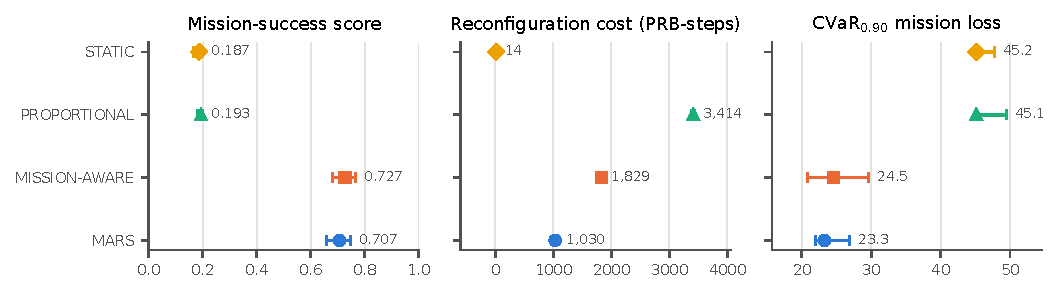
\includegraphics[width=\textwidth]{ext_ci_main.pdf}
\caption{Main metrics with 95\% bootstrap confidence intervals (30 seeds). STATIC's reconfiguration cost of 14 is the one-time move from the equal-share initial allocation.}
\label{fig:ci}
\end{figure*}

\begin{figure}[t]
\centering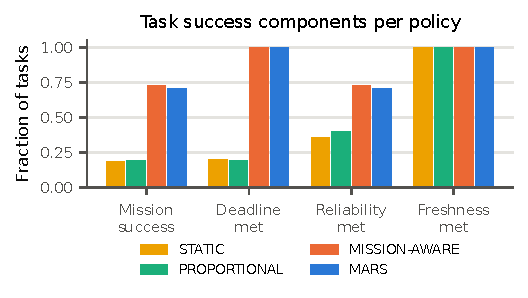
\includegraphics[width=\columnwidth]{ext_success_components.pdf}
\caption{Mean success components per policy. Freshness is satisfied in every run, so failures come from deadline or reliability checks.}
\label{fig:policy}
\end{figure}

\subsection{Paired Comparisons}
Table~\ref{tab:paired} tests MARS against each baseline seed by seed. Against STATIC and PROPORTIONAL, MARS lowers mission loss in all 30 seeds. Against MISSION-AWARE, MARS lowers reconfiguration cost in all 30 seeds (mean $-799$ PRB-steps, i.e., 43.7\%). Mission loss and success are tied in 17 seeds, better in 5, and worse in 8, and neither difference is significant. The supported claim is therefore an \emph{equivalent mission outcome at 44\% lower reconfiguration cost}, not a superior tail risk. \figref{fig:pareto} shows this separation per run.

\begin{table}[t]
\centering
\caption{Paired differences MARS $-$ baseline over 30 seeds: mean [95\% CI], win/tie/loss count for MARS, Wilcoxon signed-rank $p$.}
\label{tab:paired}
\scriptsize
\setlength{\tabcolsep}{3pt}
\begin{tabular}{llccc}
\toprule
Baseline & Metric & $\Delta$ mean [CI] & W/T/L & $p$\\
\midrule
STATIC & loss & $-26.5$ [$-27.5,-25.4$] & 30/0/0 & $<10^{-5}$\\
PROPORT. & loss & $-26.5$ [$-27.5,-25.4$] & 30/0/0 & $<10^{-5}$\\
PROPORT. & reconfig. & $-2384$ [$-2432,-2334$] & 30/0/0 & $<10^{-5}$\\
MISSION-AW. & loss & $+0.57$ [$-0.55,1.65$] & 5/17/8 & 0.23\\
MISSION-AW. & success & $-0.020$ [$-0.067,0.027$] & 5/17/8 & 0.47\\
MISSION-AW. & reconfig. & $-799$ [$-835,-762$] & 30/0/0 & $<10^{-5}$\\
\bottomrule
\end{tabular}
\end{table}

\begin{figure}[t]
\centering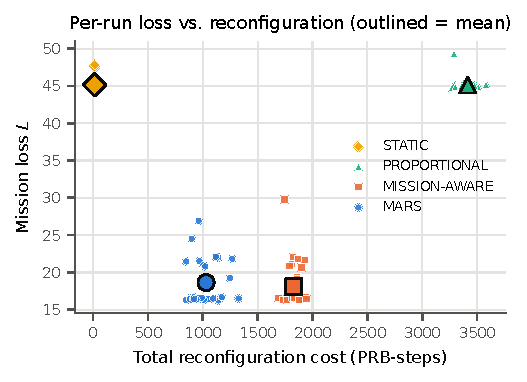
\includegraphics[width=\columnwidth]{ext_pareto.pdf}
\caption{Per-run mission loss versus reconfiguration cost (jitter $\pm0.25$ on loss). MARS and MISSION-AWARE overlap in loss but separate cleanly in cost; STATIC and PROPORTIONAL sit on the high-loss plateau.}
\label{fig:pareto}
\end{figure}

\subsection{Loss Distribution and Choice of $\beta$}
\figref{fig:tail}(a) shows the per-run loss distribution. The mission-oriented policies concentrate near 16.5 (four of five tasks succeed), and the non-adaptive policies concentrate at 45.0 (only $K_1$ succeeds). \figref{fig:tail}(b) plots CVaR$_\beta$ for $\beta\in[0,0.95]$. MARS has a higher CVaR$_\beta$ than MISSION-AWARE at every evaluated $\beta$, including the mean ($\beta=0$), except at $\beta=0.90$. The CVaR$_{0.90}$ ranking is therefore sensitive to the chosen confidence level, and we do not present it as an advantage of MARS.

\begin{figure*}[t]
\centering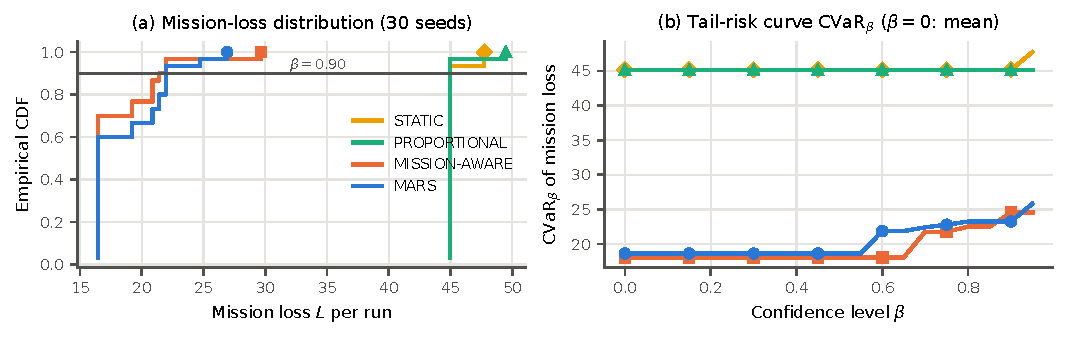
\includegraphics[width=\textwidth]{ext_loss_tail.pdf}
\caption{(a) Empirical CDF of per-run mission loss; markers show the worst run. (b) CVaR$_\beta$ as a function of $\beta$; the ranking of MARS and MISSION-AWARE changes with $\beta$.}
\label{fig:tail}
\end{figure*}

\subsection{Per-Task Anatomy and an Infeasible Task}\label{sec:k5}
\figref{fig:tasks}(a) breaks success down by task. STATIC and PROPORTIONAL complete $K_1$ and then miss the deadline of $K_2$. Each later task inherits the delay, so 80\% of their task instances fail on deadlines (\figref{fig:tasks}(b)). The mission-oriented policies meet every deadline, and their failures are reliability failures only. \figref{fig:gantt} shows the timeline for one seed.

The most important edge case is $K_5$: \emph{no policy completes valve manipulation successfully in any of the 120 runs}. $K_5$ requires $P^{\mathrm{succ}}\ge0.96$. Ignoring load and shock penalties, \eqref{eq:rel} gives $P^{\mathrm{succ}}=(0.999-0.030\sigma)(0.997-0.025\sigma)(0.998-0.020\sigma)$, which falls below 0.96 once $\sigma>0.46$. With $\sigma_0=0.6$ and positive growth, severity during $K_5$ is about 0.78, so $K_5$ is infeasible by construction for every policy. The full-mission probability is consequently zero, and the success score cannot exceed 0.8 at the nominal point. This is a property of the scenario parameters, not of the controllers, and the severity sweep confirms it: success reaches 0.96 only when $\sigma_0$ is near zero (\figref{fig:sev}).

\begin{figure*}[t]
\centering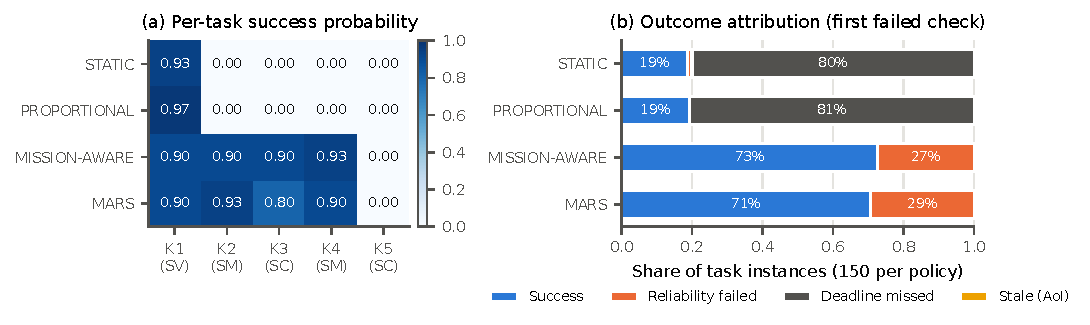
\includegraphics[width=\textwidth]{ext_task_breakdown.pdf}
\caption{(a) Per-task success probability (30 seeds). $K_5$ never succeeds. (b) Outcome of all 150 task instances per policy, attributed to the first failed check (deadline, then reliability, then freshness).}
\label{fig:tasks}
\end{figure*}

\begin{figure*}[t]
\centering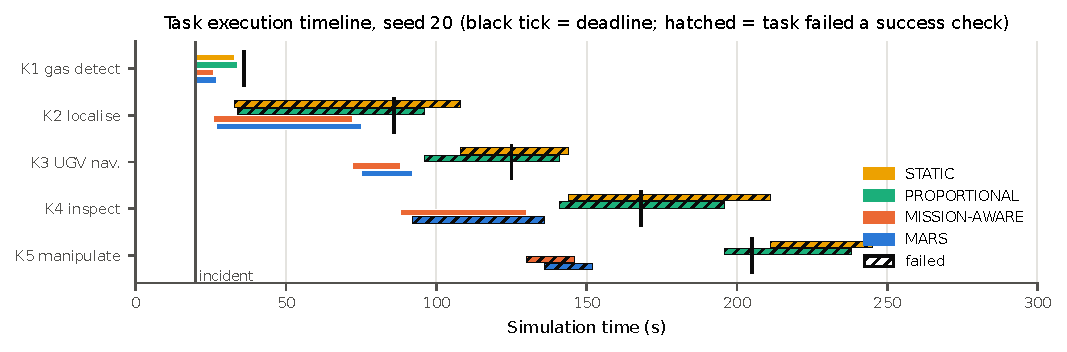
\includegraphics[width=\textwidth]{ext_gantt_seed20.pdf}
\caption{Task timeline for seed 20. Mission-oriented policies finish the mission by $t\approx150$\,s; STATIC and PROPORTIONAL overrun the $K_2$ deadline and every later deadline.}
\label{fig:gantt}
\end{figure*}

\subsection{Allocation Dynamics}
\figref{fig:trace} contrasts MISSION-AWARE and MARS on seed 20. Both move the active slice to its upper bound (60 PRBs for SC/SV, 40 for SM). MISSION-AWARE adjusts the non-active slices almost every step, whereas the MARS hold time produces piecewise-constant allocations. After the mission ends ($t>152$\,s), MARS keeps about 50 PRBs on SC because the risk reserve grows with severity. This persistent reserve explains MARS's lower control-latency proxy (\figref{fig:latency}). The proxy, $8+0.55[35-b_{\mathrm{SC}}]^++7\sigma+8\xi+\mathcal{U}(0,2.5)$\,ms, is a diagnostic only and does not enter task success. Averaged over 30 seeds, the proxy is the same for both policies while the mission runs (20.9\,ms) but 16.8 vs.\ 22.4\,ms after the mission ends. The latency advantage therefore comes from the post-mission period and does not reflect better mission service.

\begin{figure*}[t]
\centering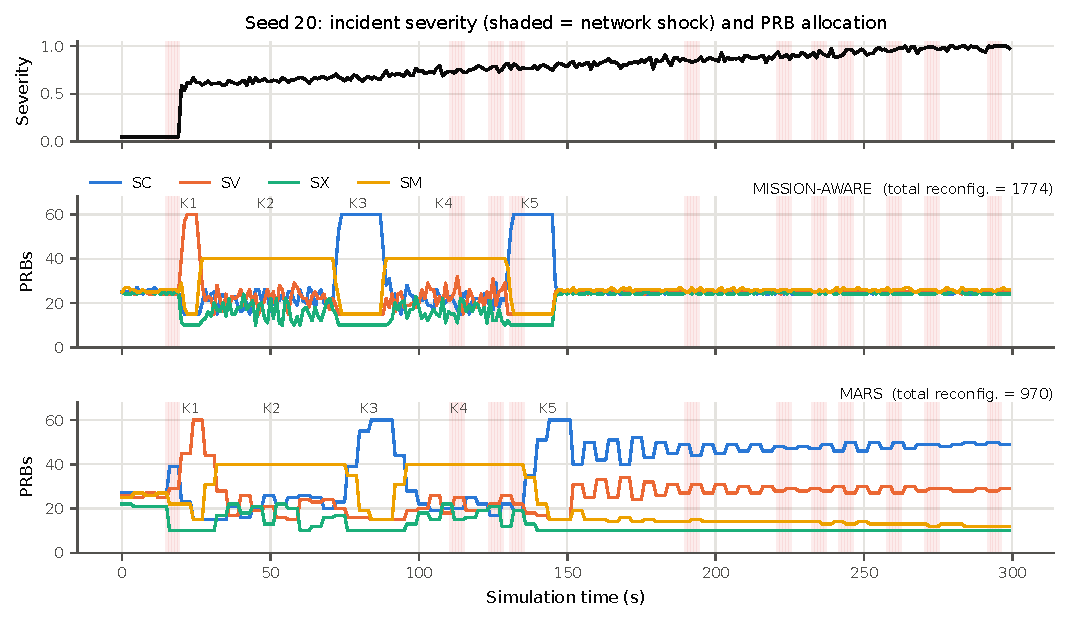
\includegraphics[width=\textwidth]{ext_trace_seed20.pdf}
\caption{Seed 20: severity with network shocks (shaded) and PRB allocation under MISSION-AWARE and MARS. Labels mark the active task.}
\label{fig:trace}
\end{figure*}

\begin{figure*}[t]
\centering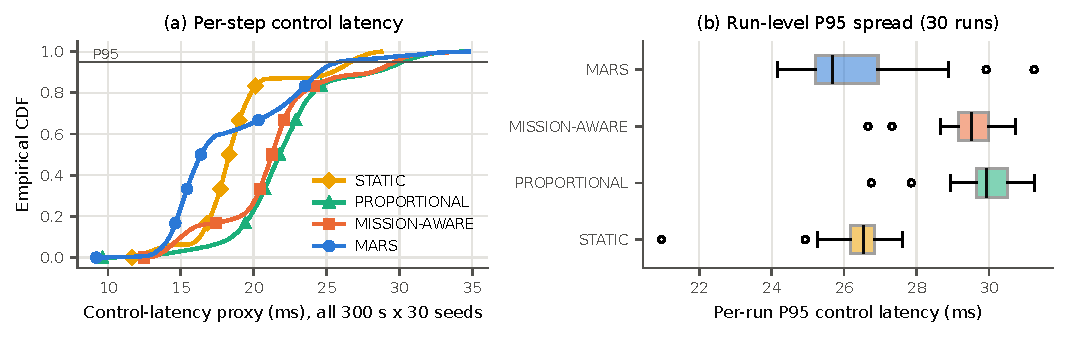
\includegraphics[width=\textwidth]{ext_latency.pdf}
\caption{(a) Per-step control-latency proxy across all runs. (b) Spread of the run-level P95. MARS's low tail arises mainly from its post-mission SC reserve. Values are model proxies, not measured NR latency.}
\label{fig:latency}
\end{figure*}

%=====================================================================
\section{Edge-Case Evaluation}\label{sec:edge}
\subsection{Radio Budget: Feasibility Floor and Surplus Paradox}
\figref{fig:prb} sweeps $B$ from 50 to 200. At $B=50=\sum_sB_s^{\min}$ every slice is pinned at its minimum, no policy can adapt, and all success scores are zero. Budgets below 50 violate \eqref{eq:prb} and are rejected by the configuration validator. Success climbs steeply between 55 and 80 PRBs for the adaptive policies, while STATIC and PROPORTIONAL need about 80 PRBs before even $K_1$ succeeds.

Counter-intuitively, success \emph{falls} for $B>120$ and returns to the STATIC level at $B\ge150$. The cause is the radio--edge coupling of \eqref{eq:edge}. The active SM slice is capped at $B^{\max}_{\mathrm{SM}}=40$ PRBs, so a larger $B$ shrinks its fraction of the edge capacity. For example, $K_2$ receives about 30\% of the edge at $B=150$ instead of 43\% at $B=100$, becomes compute-bound, and misses its deadline. MARS degrades earlier than MISSION-AWARE (0.60 vs.\ 0.70 at $B=120$): under MARS, $K_2$ misses its deadline in 13\% of runs and $K_3$ fails its reliability check in 47\%, against 0\% and 27\% for MISSION-AWARE. A deployment-grade model should decouple edge scheduling from radio share or scale $B^{\max}_s$ with $B$.

\begin{figure*}[t]
\centering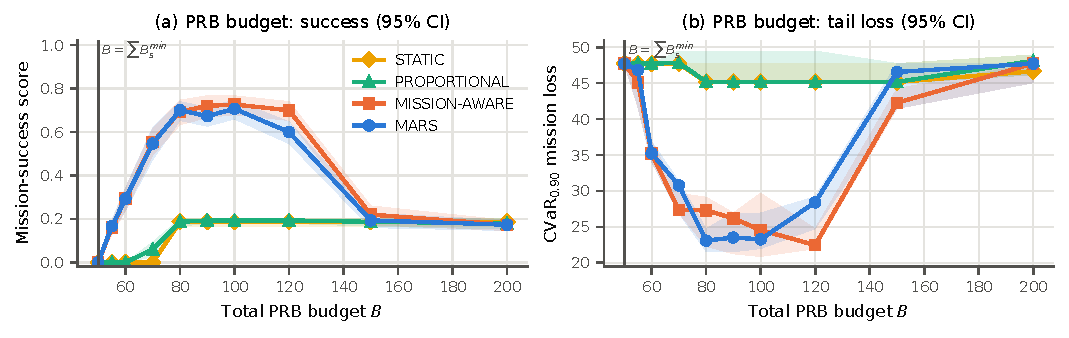
\includegraphics[width=\textwidth]{ext_sweep_prbs.pdf}
\caption{PRB-budget sweep with 95\% CIs. The vertical line marks the feasibility floor $B=\sum_s B^{\min}_s=50$. Success drops above $B=120$ because edge share is tied to radio share while the active slice is capped.}
\label{fig:prb}
\end{figure*}

\subsection{Incident Severity and Network Shocks}
\figref{fig:sev} varies $\sigma_0$. Under a benign incident, MARS reaches 0.96 [0.93, 0.99] versus 0.91 [0.85, 0.96] for MISSION-AWARE at $\sigma_0=0$, with markedly lower CVaR$_{0.90}$ (17.2 vs.\ 21.2), and 0.95 vs.\ 0.86 at $\sigma_0=0.2$. This is the regime in which $K_5$ is feasible and the protected SC slice pays off. For $\sigma_0\ge0.8$ all policies collapse: the adaptive ones to about 0.35, and STATIC and PROPORTIONAL to zero at $\sigma_0\ge0.9$, where even $K_1$ no longer succeeds.

\figref{fig:shock} sweeps the per-step shock probability. With no shocks the two mission-oriented policies coincide (0.78). Success decays smoothly as shocks become more frequent, reaching 0.13--0.16 in a shock storm ($p_{\mathrm{sh}}=0.3$). MARS's reserve gives no measurable advantage under frequent shocks.

\begin{figure*}[t]
\centering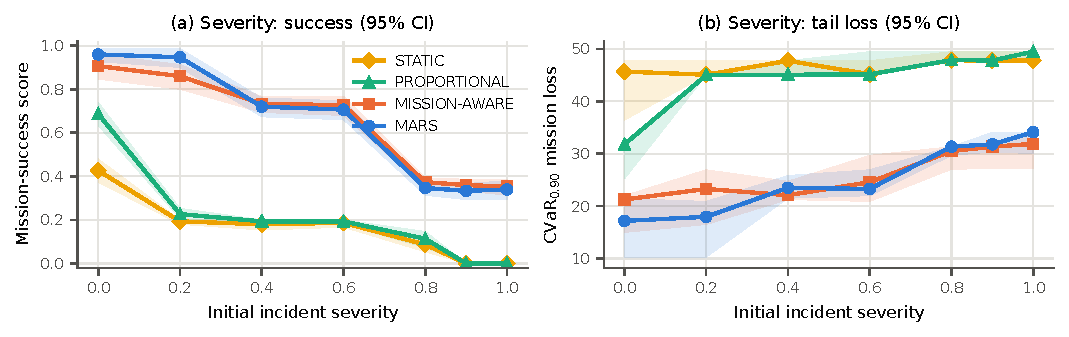
\includegraphics[width=\textwidth]{ext_sweep_severity.pdf}
\caption{Initial-severity sweep with 95\% CIs. MARS leads at low severity, where the final task becomes feasible; all policies degrade above $\sigma_0=0.6$.}
\label{fig:sev}
\end{figure*}

\begin{figure*}[t]
\centering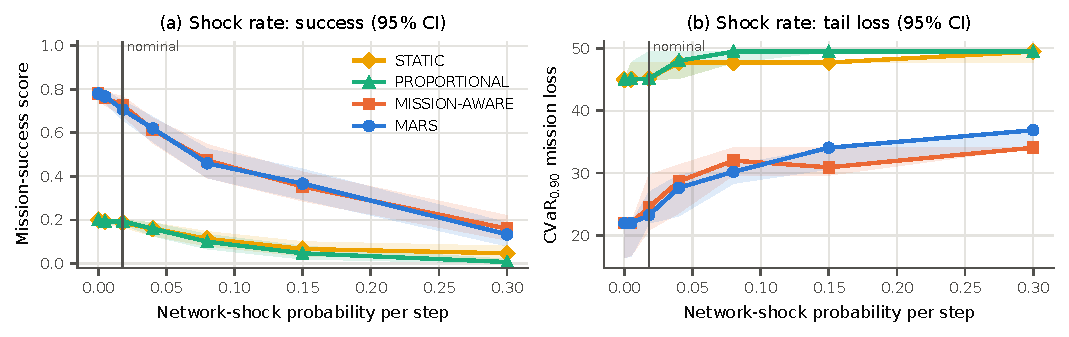
\includegraphics[width=\textwidth]{ext_sweep_shock.pdf}
\caption{Network-shock probability sweep with 95\% CIs (vertical line = nominal $p_{\mathrm{sh}}=0.018$).}
\label{fig:shock}
\end{figure*}

\subsection{Deadline Tightness and Workload}
Tightening deadlines (\figref{fig:deadline}) exposes the cost of hysteresis. At scale 0.8, MISSION-AWARE achieves 0.58 [0.52, 0.63] and MARS 0.49 [0.43, 0.53]; at 0.7 the figures are 0.36 and 0.28. At scales of 0.6 and below, at most $K_1$ succeeds under any policy. When slack is small, the 4\,s hold delays the move of PRBs to a newly activated task, and that delay cannot be recovered. Relaxed deadlines (scale 1.5) help STATIC and PROPORTIONAL most, since deadlines were their binding constraint.

Workload scaling (\figref{fig:workload}) shows the same pattern. At $1.25\times$ load MARS falls to 0.42 vs.\ 0.58 for MISSION-AWARE. Beyond $1.25\times$ success collapses for every policy (at most 0.20 at $1.5\times$). At $3\times$ load the mission no longer fits in the 300\,s horizon: the adaptive policies finish only three tasks and the rest count as failures. At light load ($\le0.5\times$) the non-adaptive policies recover to 0.4--0.6, so mission awareness matters most when resources are tight relative to workload.

\begin{figure*}[t]
\centering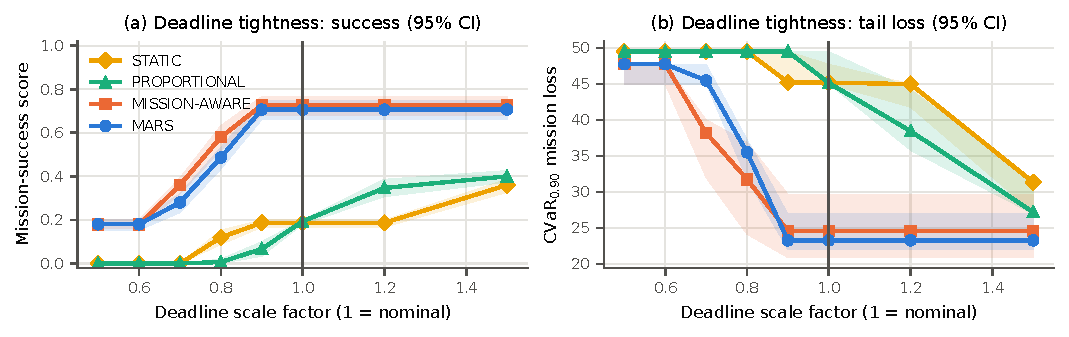
\includegraphics[width=\textwidth]{ext_sweep_deadline.pdf}
\caption{Deadline-scale sweep. At scales $\le0.6$ at most $K_1$ succeeds; between 0.7 and 0.9 MARS trails MISSION-AWARE because of its hold time.}
\label{fig:deadline}
\end{figure*}

\begin{figure*}[t]
\centering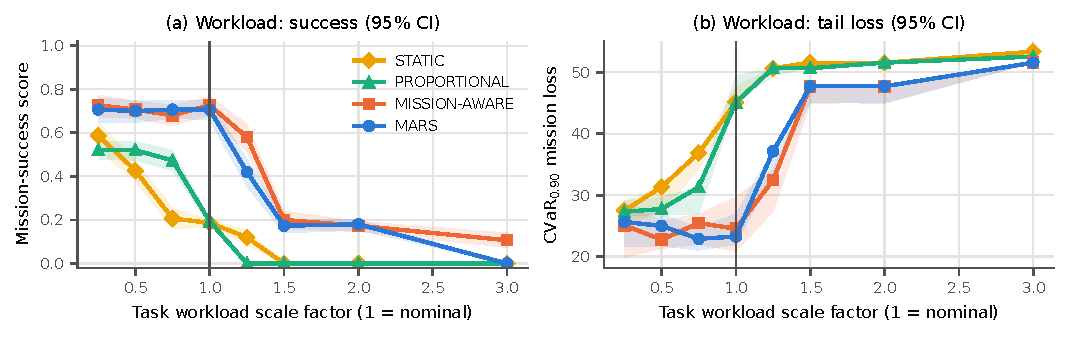
\includegraphics[width=\textwidth]{ext_sweep_workload.pdf}
\caption{Workload-scale sweep. Success collapses for every policy beyond $1.25\times$; at $3\times$ the mission no longer fits in the 300\,s horizon.}
\label{fig:workload}
\end{figure*}

\subsection{Joint Stress Map}
\figref{fig:grid} crosses severity and budget for all four policies. The mission-oriented policies match or beat the non-adaptive ones in every cell except $B=120$, $\sigma_0=0.8$, where all four policies are near 0.2, and the $B=60$, $\sigma_0=1.0$ corner, where all fail. MARS and MISSION-AWARE differ by at most 0.10 in any cell. The largest gaps are at $B=100$, $\sigma_0=0.2$ (MARS ahead, 0.95 vs.\ 0.86) and at $B=120$, $\sigma_0=0.6$ (MARS behind because of the budget paradox, 0.60 vs.\ 0.70).

\begin{figure*}[t]
\centering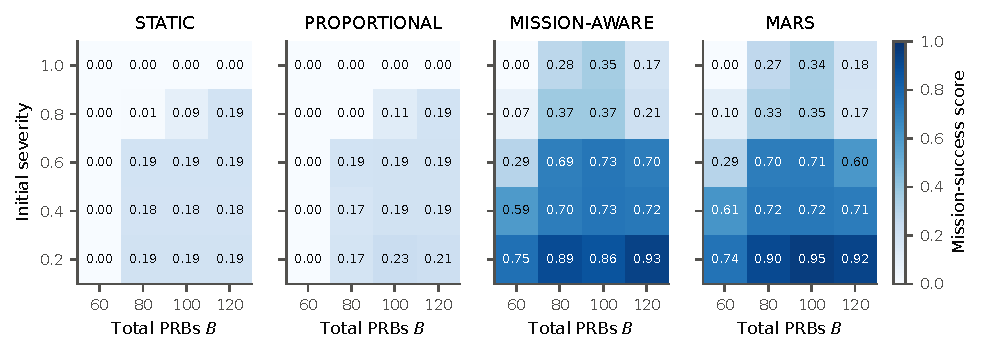
\includegraphics[width=\textwidth]{ext_stress_grid.pdf}
\caption{Mission-success score over initial severity $\times$ total PRBs (30 seeds per cell).}
\label{fig:grid}
\end{figure*}

\subsection{MARS Parameters and Ablation}\label{sec:ablation}
\figref{fig:params} sweeps the three MARS parameters. Risk aversion $\rho$ barely moves success (0.68--0.72) and changes reconfiguration cost non-monotonically. The hold time $T_h$ is the main stability lever: going from 0 to 20\,s cuts reconfiguration by $9\times$ (2908 to 327) at a cost of 0.08 in success. $T_h=0$ and $T_h=1$ behave identically because the hold condition $t-t_{\mathrm{last}}<T_h$ is never true for $T_h\le1$. A very small change limit ($\Delta_{\max}=1$) freezes adaptation (success 0.53), and $\Delta_{\max}=32$ gives the best success (0.73).

The 30-seed ablation (\figref{fig:ablation}) yields three findings.
(i) Removing AoI, urgency, or \emph{all} criticality terms gives results identical to MARS-full.
(ii) Removing hysteresis \emph{raises} success to 0.727 (it then equals MISSION-AWARE) at a $2.8\times$ higher reconfiguration cost.
(iii) Removing the risk reserve or the reconfiguration penalty \emph{lowers} reconfiguration cost (to 762 and 746) without hurting success. Because the penalty measures deviation from 25 PRBs rather than from $b_s(t-1)$, it pushes allocations toward the equal share and away from the bounds where they otherwise settle.

Saturation explains the inert criticality terms (\figref{fig:ablation}(c)). Only one task is executable at a time, so its score $\chi_k\approx8$--$23$ dominates the demand terms ($<0.35$). While the mission runs on seed 20 ($t=20$--$152$\,s), the largest softmax weight is at least 0.9997 at every step. The resulting target exceeds the slice's upper bound and is clipped, so the allocation depends only on \emph{which} slice is active, not on \emph{how} critical it is. Making the criticality weights matter requires concurrent tasks or a softmax temperature that keeps scores in the unsaturated range.

\begin{figure*}[t]
\centering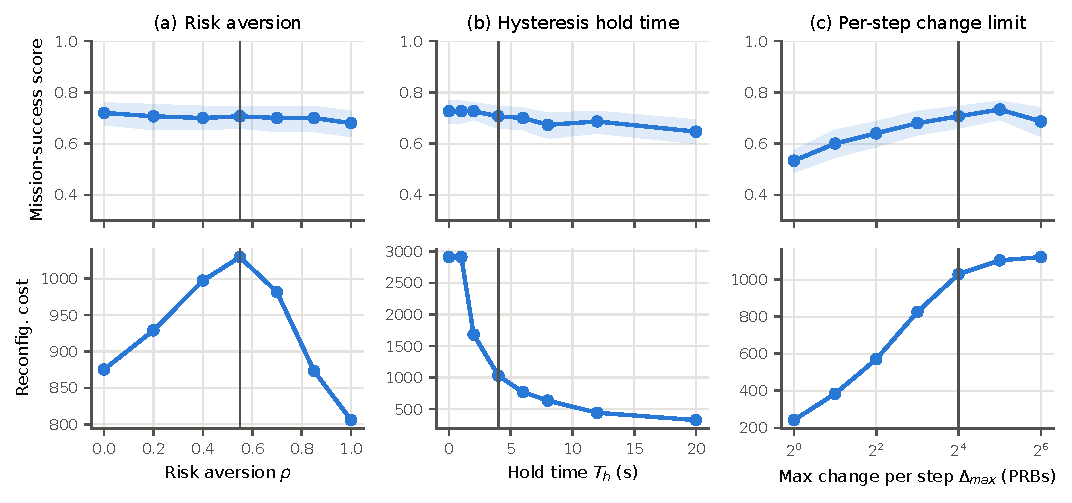
\includegraphics[width=\textwidth]{ext_mars_params.pdf}
\caption{MARS parameter sensitivity (30 seeds; vertical line = nominal). Top: success with 95\% CI. Bottom: reconfiguration cost.}
\label{fig:params}
\end{figure*}

\begin{figure*}[t]
\centering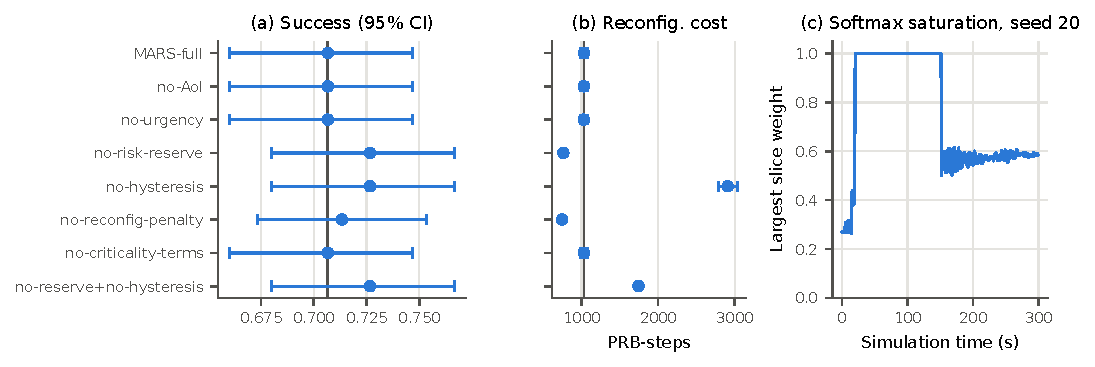
\includegraphics[width=\textwidth]{ext_ablation.pdf}
\caption{(a,b) Ablation over 30 seeds with 95\% CIs (vertical line = MARS-full). AoI, urgency, and all criticality terms have no effect; removing hysteresis increases success but nearly triples reconfiguration. (c) Largest MARS slice weight per step on seed 20: it is saturated at 1 for the whole mission, so slice bounds, not criticality values, set the allocation.}
\label{fig:ablation}
\end{figure*}

%=====================================================================
\section{Discussion and Limitations}
\textbf{What the evidence supports.} (1) Mission-aware allocation is far better than fixed or demand-proportional slicing in this model. The effect holds in every paired seed and across the stress map except degenerate corners. (2) MARS delivers the same nominal mission outcome as MISSION-AWARE with 44\% less reconfiguration, which matters where each reallocation carries signalling or instability cost. (3) MARS is clearly better under mild incidents.

\textbf{What it does not support.} MARS has no statistically supported tail-risk advantage at the nominal point, and its CVaR ranking depends on $\beta$. Under tight deadlines, heavy workload, or surplus PRBs it is worse than MISSION-AWARE, because the hold time and reserve trade agility for stability. The criticality score \eqref{eq:criticality} does not influence decisions in the current single-task-at-a-time configuration.

\textbf{Design implications.} An adaptive hold time that shrinks when deadline slack is small would combine the stability of MARS at nominal load with the agility of MISSION-AWARE under pressure. A reconfiguration penalty relative to $b_s(t-1)$, a reserve that switches off when the mission ends, and an edge scheduler independent of radio share would remove the three model artifacts identified above.

\textbf{Threats to validity.} \emph{Internal:} results depend on hand-chosen parameters, and several conclusions (e.g., $K_5$ infeasibility and the budget paradox) follow directly from modelling choices that we expose rather than tune away. Thirty seeds give wide CVaR$_{0.90}$ intervals because only three runs fall in the tail. \emph{Construct:} the success score is a per-task fraction, not mission completion; latency values are proxies outside task success; mission loss uses $w_k(1+0.25h_k)$ rather than $\chi_k$. \emph{External:} the radio model is analytical, with one cell, one edge server, no mobility or handover, and independent component reliabilities. No packet-level, testbed, or field validation has been performed, and no E2/A1 interface is exercised. MARS is not compared against an optimization-based or learning-based controller.

%=====================================================================
\section{Conclusion}
MARS-O-RAN links a five-task emergency mission to four network slices and evaluates task success, deadlines, freshness, reliability, reconfiguration, and tail loss in a reproducible digital twin. We formulated mission-aware slicing as a stochastic integer program and proposed MARS, a heuristic that approximates its objective with a criticality score, a risk reserve, and stability rules. A paired statistical analysis and eleven edge-case studies give a more precise picture than aggregate means. Mission-aware slicing is robustly beneficial. The MARS stability mechanisms cut reconfiguration by 44\% at equal nominal outcome and help under mild incidents, but they cost agility when slack is tight. The edge cases also uncovered an infeasible final task, a radio--edge budget paradox, and saturated criticality weights. Future work will validate the abstractions with ns-3/5G-LENA \cite{lena}, recalibrate the reliability model so every task is feasible at nominal severity, introduce concurrent tasks, implement an adaptive hold time, and benchmark against a CVaR-constrained mixed-integer program and a reinforcement-learning controller.

\section*{Reproducibility}
The code, configuration files, and synthetic data generator are provided with this paper. \texttt{src/run\_all.py} runs the main experiment, \texttt{src/edge\_case\_experiments.py} computes statistics, sweeps, and all figures with fixed seeds, and \texttt{src/verify\_paper\_claims.py} recomputes every number quoted in the text.

\begin{thebibliography}{00}
\bibitem{oranarch} O-RAN Software Community, ``O-RAN Architecture Overview,'' F-Release documentation. [Online]. Available: \url{https://docs.o-ran-sc.org/en/f-release/architecture/architecture.html}. Accessed: Oct. 15, 2026.
\bibitem{oranwg3} O-RAN ALLIANCE, ``Near-Real-time RAN Intelligent Controller and E2 Interface Workgroup (WG3).'' [Online]. Available: \url{https://www.o-ran.org/technical-groups/wg3}. Accessed: Oct. 15, 2026.
\bibitem{polese} M. Polese, L. Bonati, S. D'Oro, S. Basagni, and T. Melodia, ``Understanding O-RAN: Architecture, interfaces, algorithms, security, and research challenges,'' \emph{IEEE Commun. Surveys Tuts.}, vol. 25, no. 2, pp. 1376--1411, 2023, doi: 10.1109/COMST.2023.3239220.
\bibitem{safeslice} A. M. Nagib, H. Abou-Zeid, and H. S. Hassanein, ``SafeSlice: Enabling SLA-compliant O-RAN slicing via safe deep reinforcement learning,'' in \emph{Proc. IEEE Int. Conf. Mach. Learn. Commun. Netw. (ICMLCN)}, 2025, arXiv:2503.12753.
\bibitem{bvlos} P. Baguer, E. Municio, G. Garcia-Aviles, and X. Costa-Perez, ``Enabling beyond-visual-line-of-sight drones operation over Open RAN 5G networks with slicing,'' \emph{IEEE Netw.}, vol. 38, no. 6, pp. 163--169, Nov. 2024, doi: 10.1109/MNET.2024.3420085.
\bibitem{kaul} S. Kaul, R. Yates, and M. Gruteser, ``Real-time status: How often should one update?'' in \emph{Proc. IEEE INFOCOM}, 2012, pp. 2731--2735.
\bibitem{aoi} R. D. Yates, Y. Sun, D. R. Brown III, S. K. Kaul, E. Modiano, and S. Ulukus, ``Age of information: An introduction and survey,'' \emph{IEEE J. Sel. Areas Commun.}, vol. 39, no. 5, pp. 1183--1210, May 2021, doi: 10.1109/JSAC.2021.3065072.
\bibitem{polyanskiy} Y. Polyanskiy, H. V. Poor, and S. Verd\'u, ``Channel coding rate in the finite blocklength regime,'' \emph{IEEE Trans. Inf. Theory}, vol. 56, no. 5, pp. 2307--2359, May 2010, doi: 10.1109/TIT.2010.2043769.
\bibitem{cvar} R. T. Rockafellar and S. Uryasev, ``Optimization of conditional value-at-risk,'' \emph{J. Risk}, vol. 2, no. 3, pp. 21--41, 2000, doi: 10.21314/JOR.2000.038.
\bibitem{lena} N. Patriciello, S. Lag\'en, B. Bojovi\'c, and L. Giupponi, ``An E2E simulator for 5G NR networks,'' \emph{Simul. Model. Pract. Theory}, vol. 96, Art. no. 101933, 2019, doi: 10.1016/j.simpat.2019.101933.
\bibitem{bootstrap} B. Efron and R. J. Tibshirani, \emph{An Introduction to the Bootstrap}. New York, NY, USA: Chapman \& Hall, 1993.
\bibitem{wilcoxon} F. Wilcoxon, ``Individual comparisons by ranking methods,'' \emph{Biometrics Bull.}, vol. 1, no. 6, pp. 80--83, 1945, doi: 10.2307/3001968.
\end{thebibliography}
\end{document}
